\section{Non-Uniformity of the Decision Tree Model}
\label{tree:sorting:nonuniformity}

\begin{figure}
\center
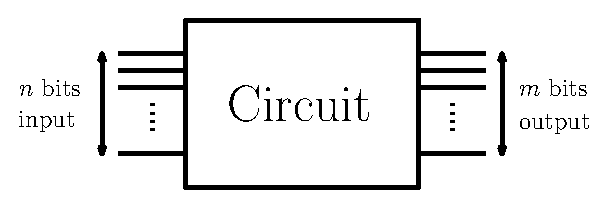
\includegraphics[height=0.2\textheight]{fig/sorting/model/circuit}
\caption{A boolean circuit with \(n\) bits of input and \(m\) bits of output.}
\label{fig:sorting:nonuniformity:circuit}
\end{figure}

A non-uniform model of computation is a model where inputs of different
lengths can be processed by different algorithms. In this section we show that
our model is non-uniform. An example of such a model is circuit complexity. An
electronic circuit can be seen as an algorithm with fixed size input and fixed
size output. In contrast with models equivalent to the Universal Turing
Machine, where one algorithm can solve an input of any size, in this model we
will need one circuit per possible size of the input.

Since we want to solve problems of any size, to each computational problem we
will assign a family of boolean circuits \(C_1,C_2,\ldots\) that solve
instances of the problem for every possible input size. We will say that this
circuit family is P-uniform if there exists a Turing machine running in
polynomial-time in \(n\), where \(n\) is the input and \(C_n\) is the output.

As a general fact, we can design an algorithm for any problem in the decision
tree model with fixed input size \(n\) and fixed output set \(\Gamma\) using
the following approach. We generate the finite set containing all possible
decision trees with \(\card{\Gamma}\) leaves. To each node of the trees we
generated corresponds a query of the form \(q(x_1,\ldots,x_n)\) where
\((x_1,\ldots,x_n)\) is the input vector. We then keep the decision tree with
minimal height \(h\). To solve an instance of size \(n\) we can just walk
through the decision tree we built, branching according to the answers we get
from the queries. This is equivalent to build \(C_n\), a circuit of depth
\(h\). For problems where \(\card{\Gamma}\) is at most singly exponential in
\(n\), \(h\) will be polynomial and thus for each problem size we have a
circuit \(C_n\) giving the correct output in polynomial time. Unfortunately,
there exist problems for which this approach will take exponential time in
\(n\) to construct \(C_n\) while \(h\) is polynomial, hence the circuit
families for those problems are not P-uniform and the decision tree model is
non-uniform.

For all of the problems we will study, one can make the parallel between the
complexity analysis on the number of comparisons required to solve those
problems and an analysis of the complexity of those problems in the non-uniform
boolean circuit model.
